%%%%%%%%%%%%%%%%%%%%%%%%%%%%%%%%%%%%%%%%%
% Beamer Presentation
% LaTeX Template
% Version 1.0 (10/11/12)
%
% This template has been downloaded from:
% http://www.LaTeXTemplates.com
%
% License:
% CC BY-NC-SA 3.0 (http://creativecommons.org/licenses/by-nc-sa/3.0/)
%
%%%%%%%%%%%%%%%%%%%%%%%%%%%%%%%%%%%%%%%%%

%----------------------------------------------------------------------------------------
%	PACKAGES AND THEMES
%----------------------------------------------------------------------------------------

\documentclass[UTF8,aspectratio=169,14pt]{ctexbeamer}

\usepackage{hyperref}
\hypersetup{
	colorlinks=true,
	linkcolor=red,
	anchorcolor=blue,
	citecolor=green
}

\mode<presentation> {
	
	% The Beamer class comes with a number of default slide themes
	% which change the colors and layouts of slides. Below this is a list
	% of all the themes, uncomment each in turn to see what they look like.
	
	%\usetheme{default}
	%\usetheme{AnnArbor}
	%\usetheme{Antibes}
	%\usetheme{Bergen}
	%\usetheme{Berkeley}
	%\usetheme{Berlin}
	%\usetheme{Boadilla}
	%\usetheme{CambridgeUS}
	%\usetheme{Copenhagen}
	%\usetheme{Darmstadt}
	%\usetheme{Dresden}
	%\usetheme{Frankfurt}
	%\usetheme{Goettingen}
	%\usetheme{Hannover}
	%\usetheme{Ilmenau}
	%\usetheme{JuanLesPins}
	%\usetheme{Luebeck}
	\usetheme{Madrid}
	%\usetheme{Malmoe}
	%\usetheme{Marburg}
	%\usetheme{Montpellier}
	%\usetheme{PaloAlto}
	%\usetheme{Pittsburgh}
	%\usetheme{Rochester}
	%\usetheme{Singapore}
	%\usetheme{Szeged}
	%\usetheme{Warsaw}
	
	% As well as themes, the Beamer class has a number of color themes
	% for any slide theme. Uncomment each of these in turn to see how it
	% changes the colors of your current slide theme.
	
	%\usecolortheme{albatross}
	%\usecolortheme{beaver}
	%\usecolortheme{beetle}
	%\usecolortheme{crane}
	%\usecolortheme{dolphin}
	%\usecolortheme{dove}
	%\usecolortheme{fly}
	%\usecolortheme{lily}
	%\usecolortheme{orchid}
	%\usecolortheme{rose}
	%\usecolortheme{seagull}
	%\usecolortheme{seahorse}
	%\usecolortheme{whale}
	%\usecolortheme{wolverine}
	
	%\setbeamertemplate{footline} % To remove the footer line in all slides uncomment this line
	%\setbeamertemplate{footline}[page number] % To replace the footer line in all slides with a simple slide count uncomment this line
	
	%\setbeamertemplate{navigation symbols}{} % To remove the navigation symbols from the bottom of all slides uncomment this line
}

\usepackage{graphicx} % Allows including images
\graphicspath{{./figs/}}
\usepackage{booktabs} % Allows the use of \toprule, \midrule and \bottomrule in tables
\usepackage{longtable}
\usepackage{listings}
\usepackage{xcolor}
\lstset{numbers=left, %设置行号位置
	numberstyle=\tiny, %设置行号大小
	keywordstyle=\color{blue}, %设置关键字颜色
	commentstyle=\color[cmyk]{1,0,1,0}, %设置注释颜色
	frame=single, %设置边框格式
	escapeinside=``, %逃逸字符(1左面的键),用于显示中文
	%breaklines, %自动折行
	extendedchars=false, %解决代码跨页时,章节标题,页眉等汉字不显示的问题
	xleftmargin=2em,xrightmargin=2em, aboveskip=1em, %设置边距
	tabsize=4, %设置tab空格数
	showspaces=false %不显示空格
}
% Fonts
% \usepackage{libertine}
% \setmonofont{Courier}
\setCJKsansfont[ItalicFont=Noto Serif CJK SC Black, BoldFont=Noto Sans CJK SC Black]{Noto Sans CJK SC}


%----------------------------------------------------------------------------------------
%	TITLE PAGE
%----------------------------------------------------------------------------------------

\title[第1讲]{第1讲 :操作系统概述} % The short title appears at the bottom of every slide, the full title is only on the title page
\subtitle{第六节:操作系统历史}
\author{向勇、陈渝} % Your name
\institute[清华大学] % Your institution as it will appear on the bottom of every slide, may be shorthand to save space
{
清华大学计算机系 \\ % Your institution for the title page
\medskip
\textit{xyong,yuchen@tsinghua.edu.cn} % Your email address
}
\date{\today} % Date, can be changed to a custom date

\begin{document}

\begin{frame}
\titlepage % Print the title page as the first slide
\end{frame}

\begin{frame}
\frametitle{提纲} % Table of contents slide, comment this block out to remove it
\tableofcontents % Throughout your presentation, if you choose to use \section{} and \subsection{} commands, these will automatically be printed on this slide as an overview of your presentation
\end{frame}

%----------------------------------------------------------------------------------------
%	PRESENTATION SLIDES
%----------------------------------------------------------------------------------------

%------------------------------------------------
\section{第六节:操作系统历史} % Sections can be created in order to organize your presentation into discrete blocks, all sections and subsections are automatically printed in the table of contents as an overview of the talk
%------------------------------------------------
\subsection{单用户系统}
\subsection{批处理系统}
\subsection{多道程序系统}
\subsection{分时系统}
\subsection{个人计算机}
\subsection{分布式计算}

\begin{frame}

\frametitle{单用户系统}

单用户系统(1945-1955)
\begin{itemize}
\item 手动连线/纸带传输进行程序输入
\item 机器成本远大于人力成本	
\item 操作系统=装载器(loader)+程序库(libraries)
\item 问题:昂贵组件的低利用率
\end{itemize}

	\begin{figure}
	\centering
	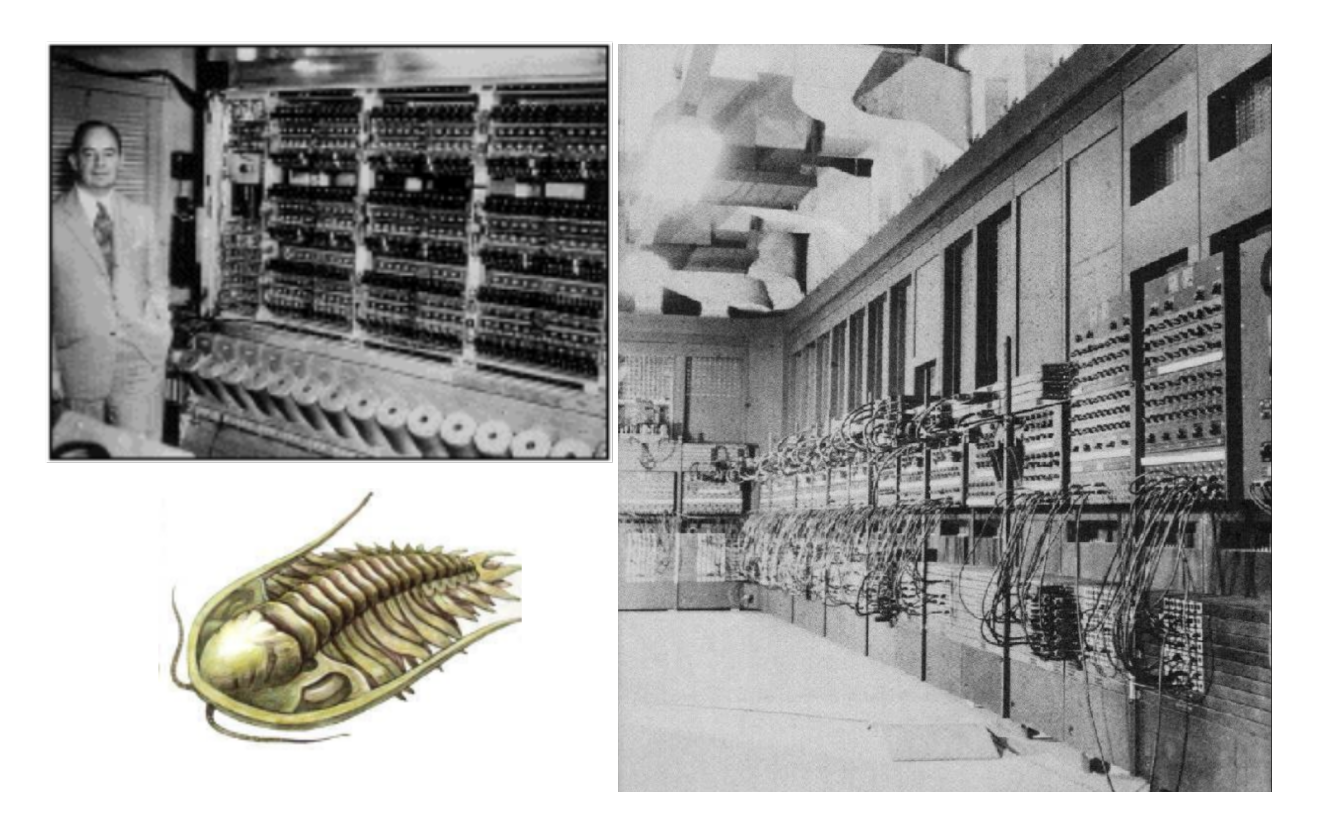
\includegraphics[width=0.6\linewidth]{history-single-user-system}
	\caption{单用户系统}
\end{figure}

\end{frame}



\begin{frame}
	
	\frametitle{批处理系统}
	
	批处理系统(1955-1965)
	\begin{itemize}
		\item 磁带/磁盘传输进行程序输入
		\item 机器成本大于人力成本	
		\item 操作系统=装载器(loader)+程序控制器(sequencer)+输出处理器(output processor)
		\item 问题:相比以前利用率提高
	\end{itemize}
	
	\begin{figure}
		\centering
		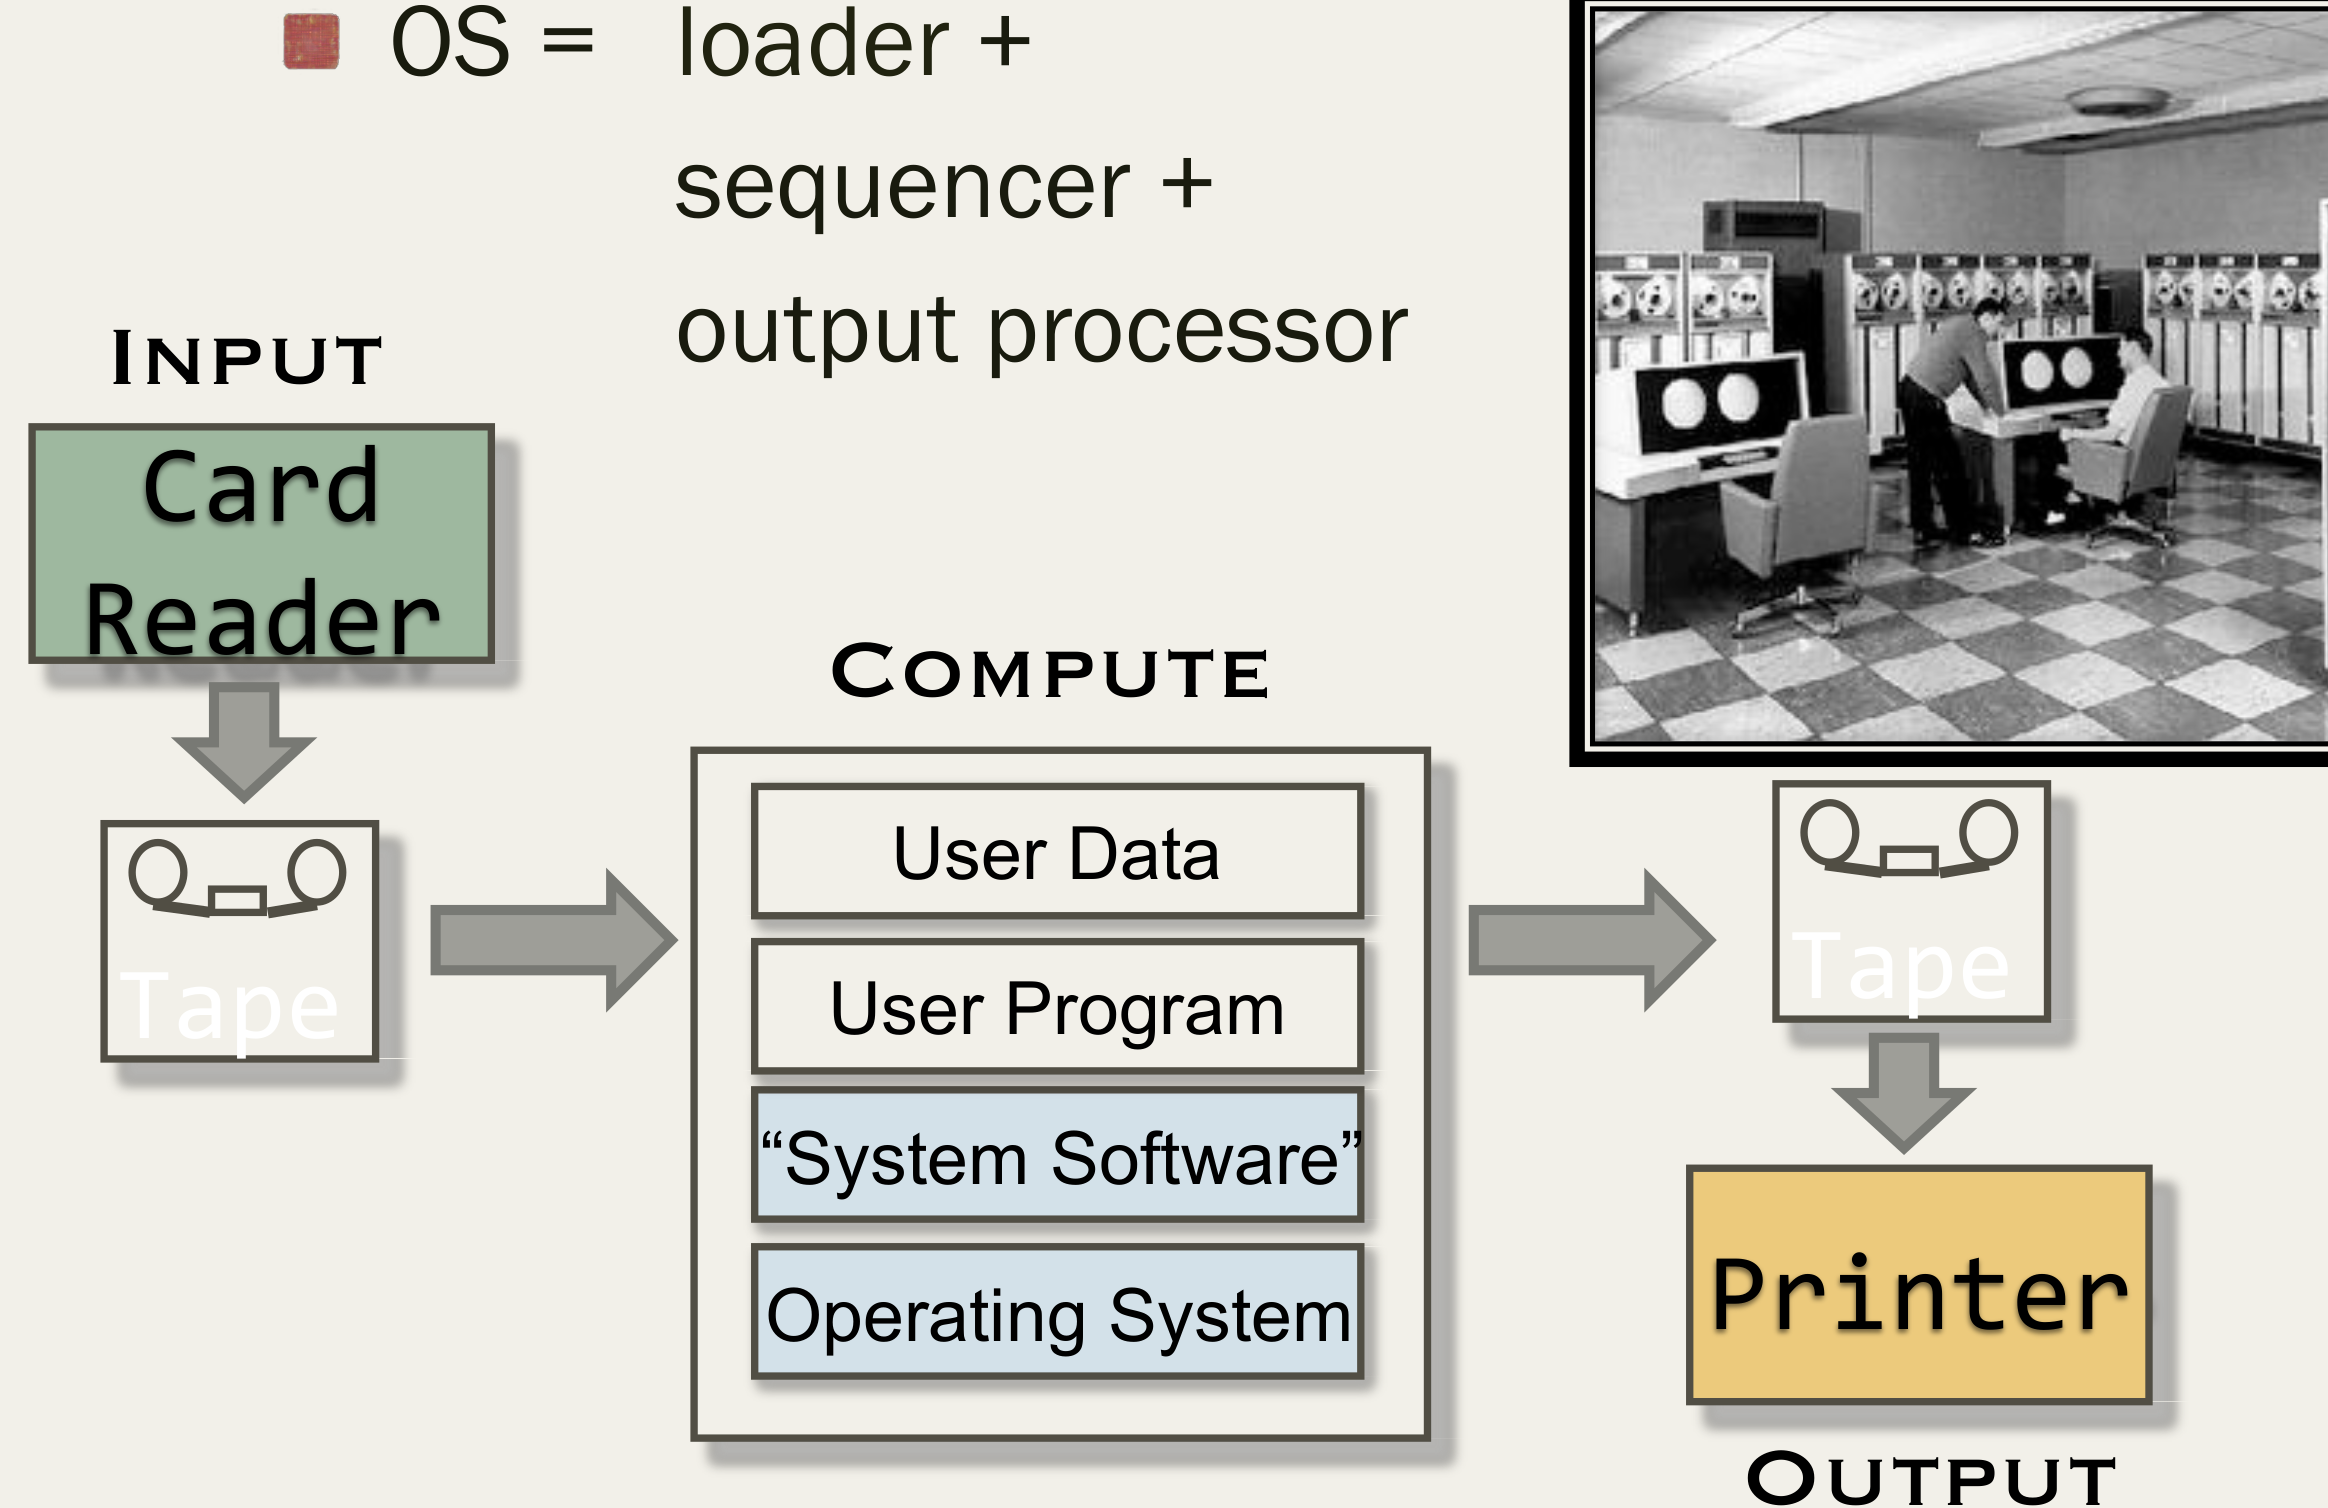
\includegraphics[width=0.6\linewidth]{history-batch-processing}
		\caption{批处理系统}
	\end{figure}
	
\end{frame}

\begin{frame}
	
	\frametitle{批处理系统}
	
	批处理系统(1955-1965)
	\begin{itemize}
		\item 磁带/磁盘传输进行程序输入
		\item 机器成本大于人力成本	
		\item 操作系统=装载器(loader)+程序控制器(sequencer)+输出处理器(output processor)
		\item 演变:相比以前利用率提高
	\end{itemize}
	
	\begin{figure}
		\centering
		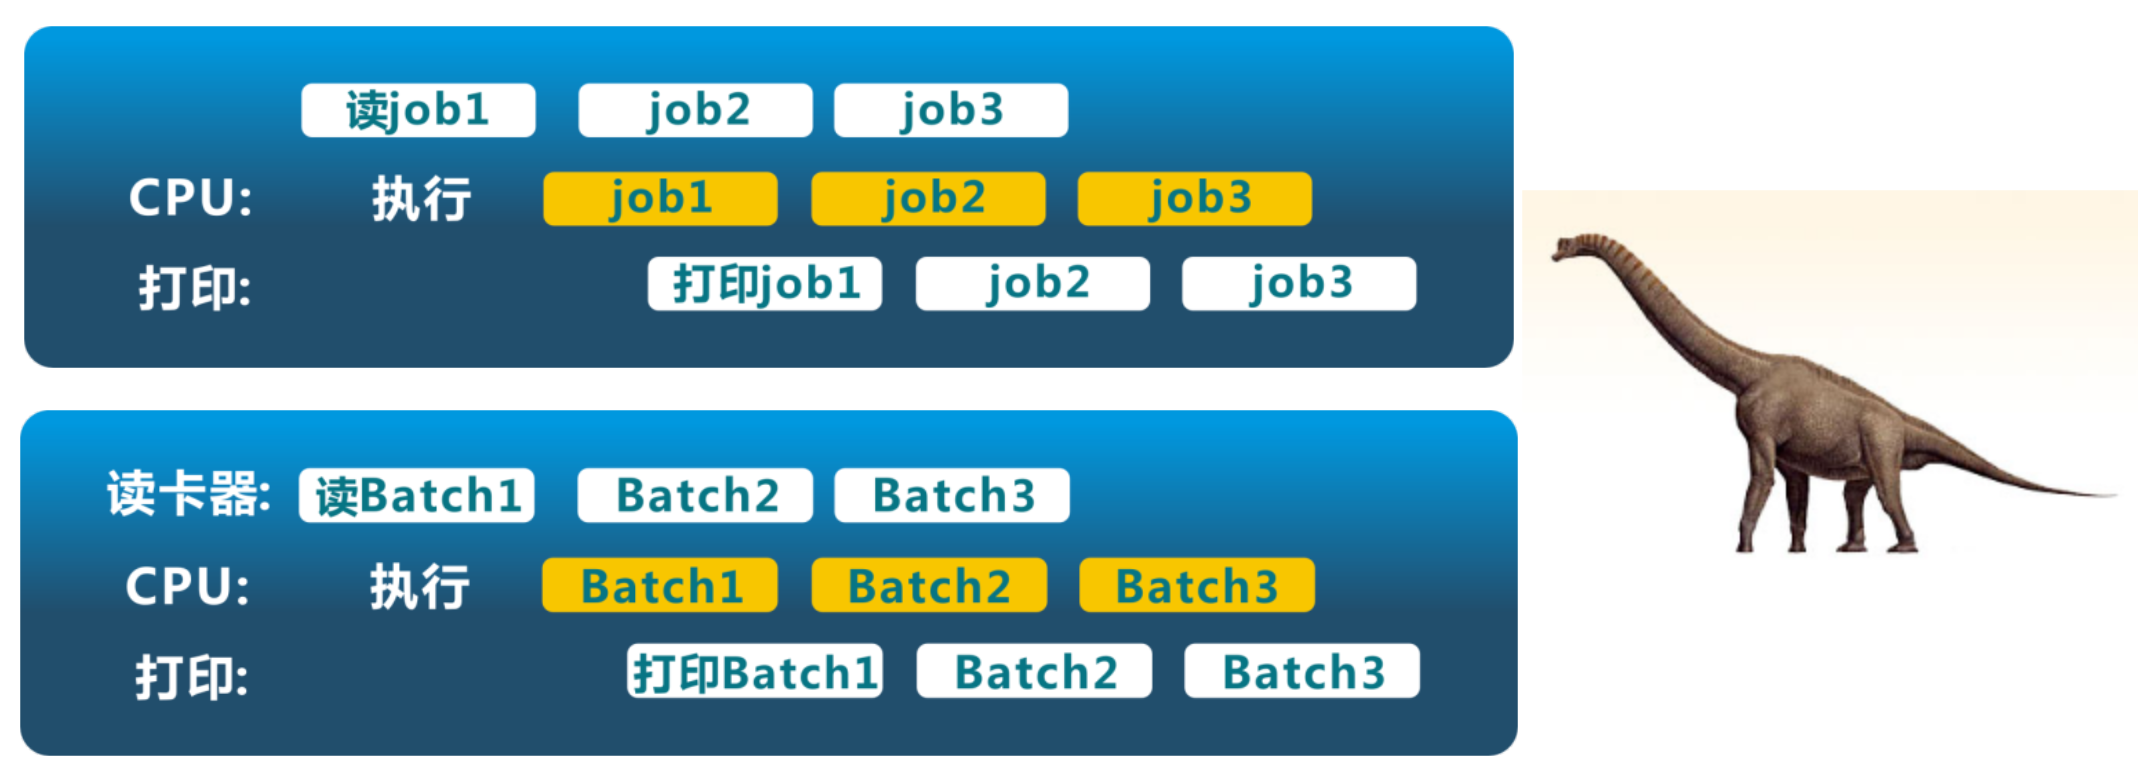
\includegraphics[width=0.6\linewidth]{history-batch-process-graph}
		\caption{批处理流程}
	\end{figure}
	
\end{frame}




\begin{frame}
	
	\frametitle{多道程序系统}
	
	多道程序系统(1955-1980)
	\begin{itemize}
		\item 多个程序驻留内存中
		\item 多个程序轮流使用CPU	
		\item 操作系统=装载器+程序调度+内存管理+输出管理
		\item 演变:相比以前利用率提高
	\end{itemize}
	
	\begin{figure}
		\centering
		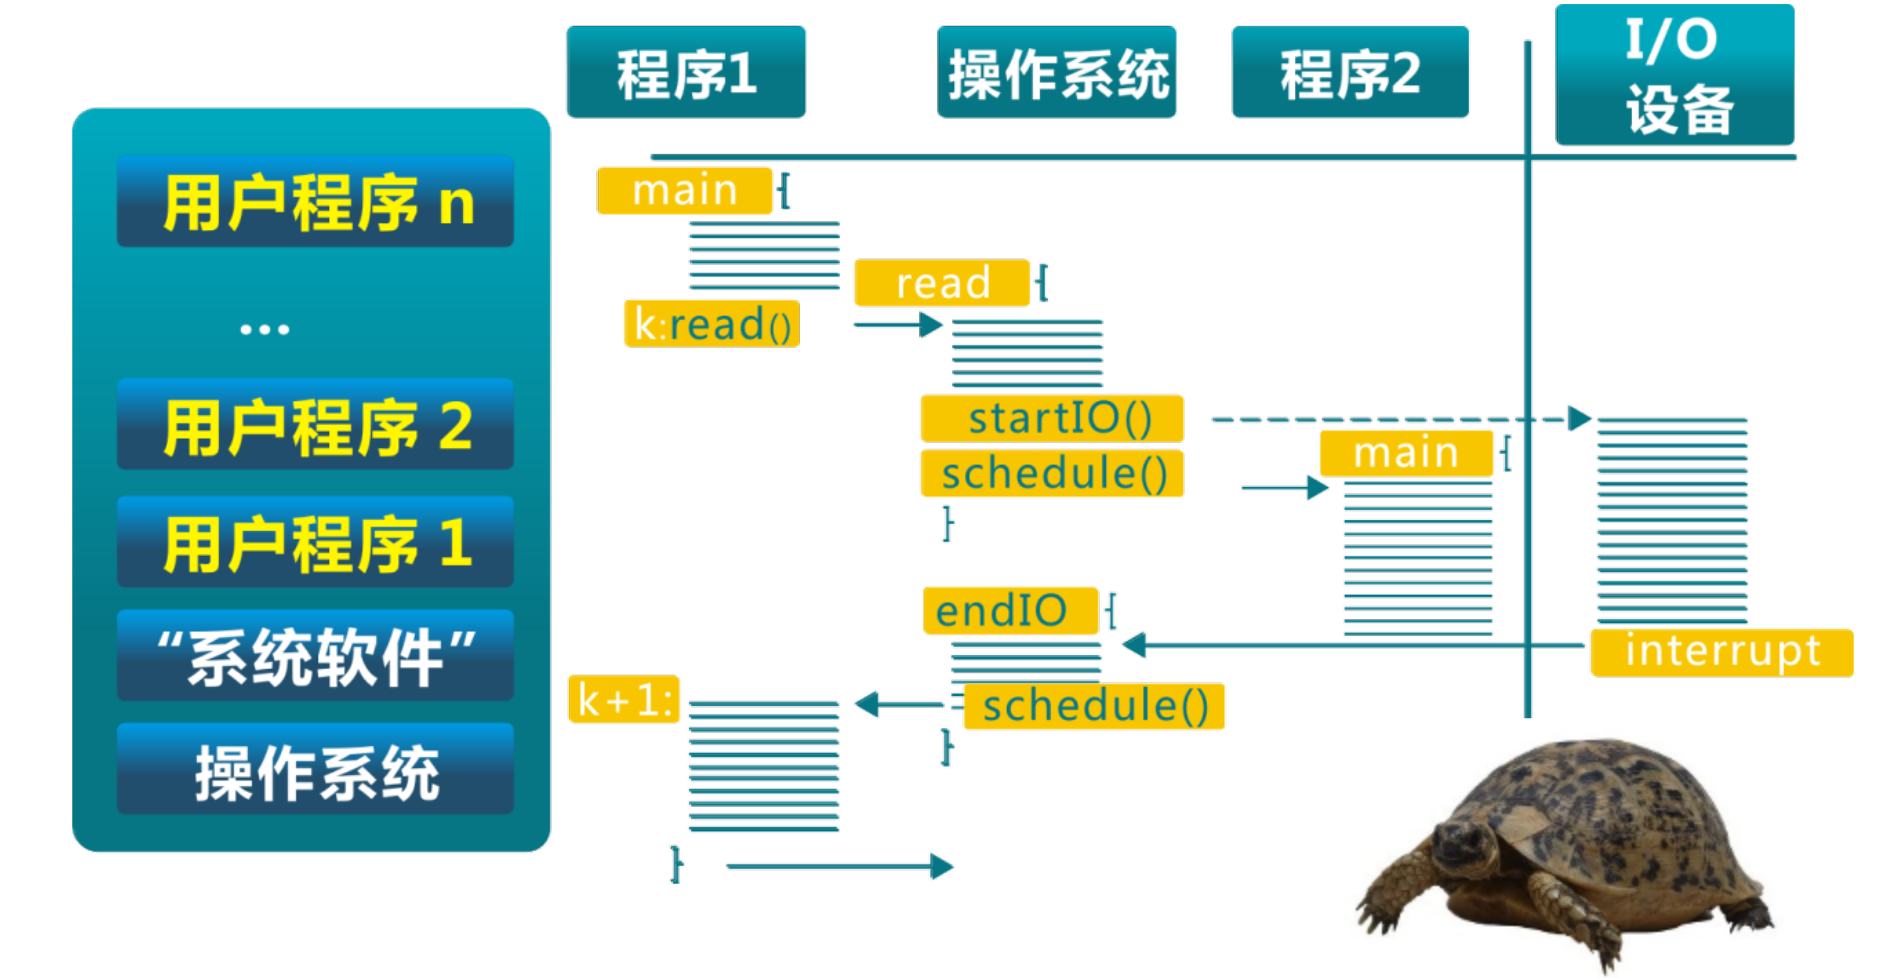
\includegraphics[width=0.7\linewidth]{history-multiprogramming}
		\caption{多道程序处理流程}
	\end{figure}
	
\end{frame}


\begin{frame}
	
	\frametitle{分时系统}
	
	分时系统(1970- )
	\begin{itemize}
		\item 多个程序驻留内存中
		\item 多个程序分时使用CPU	
		\item 操作系统=装载器+程序调度+内存管理+中断处理+...
		\item 演变:相比以前利用率提高
	\end{itemize}
	
	\begin{figure}
		\centering
		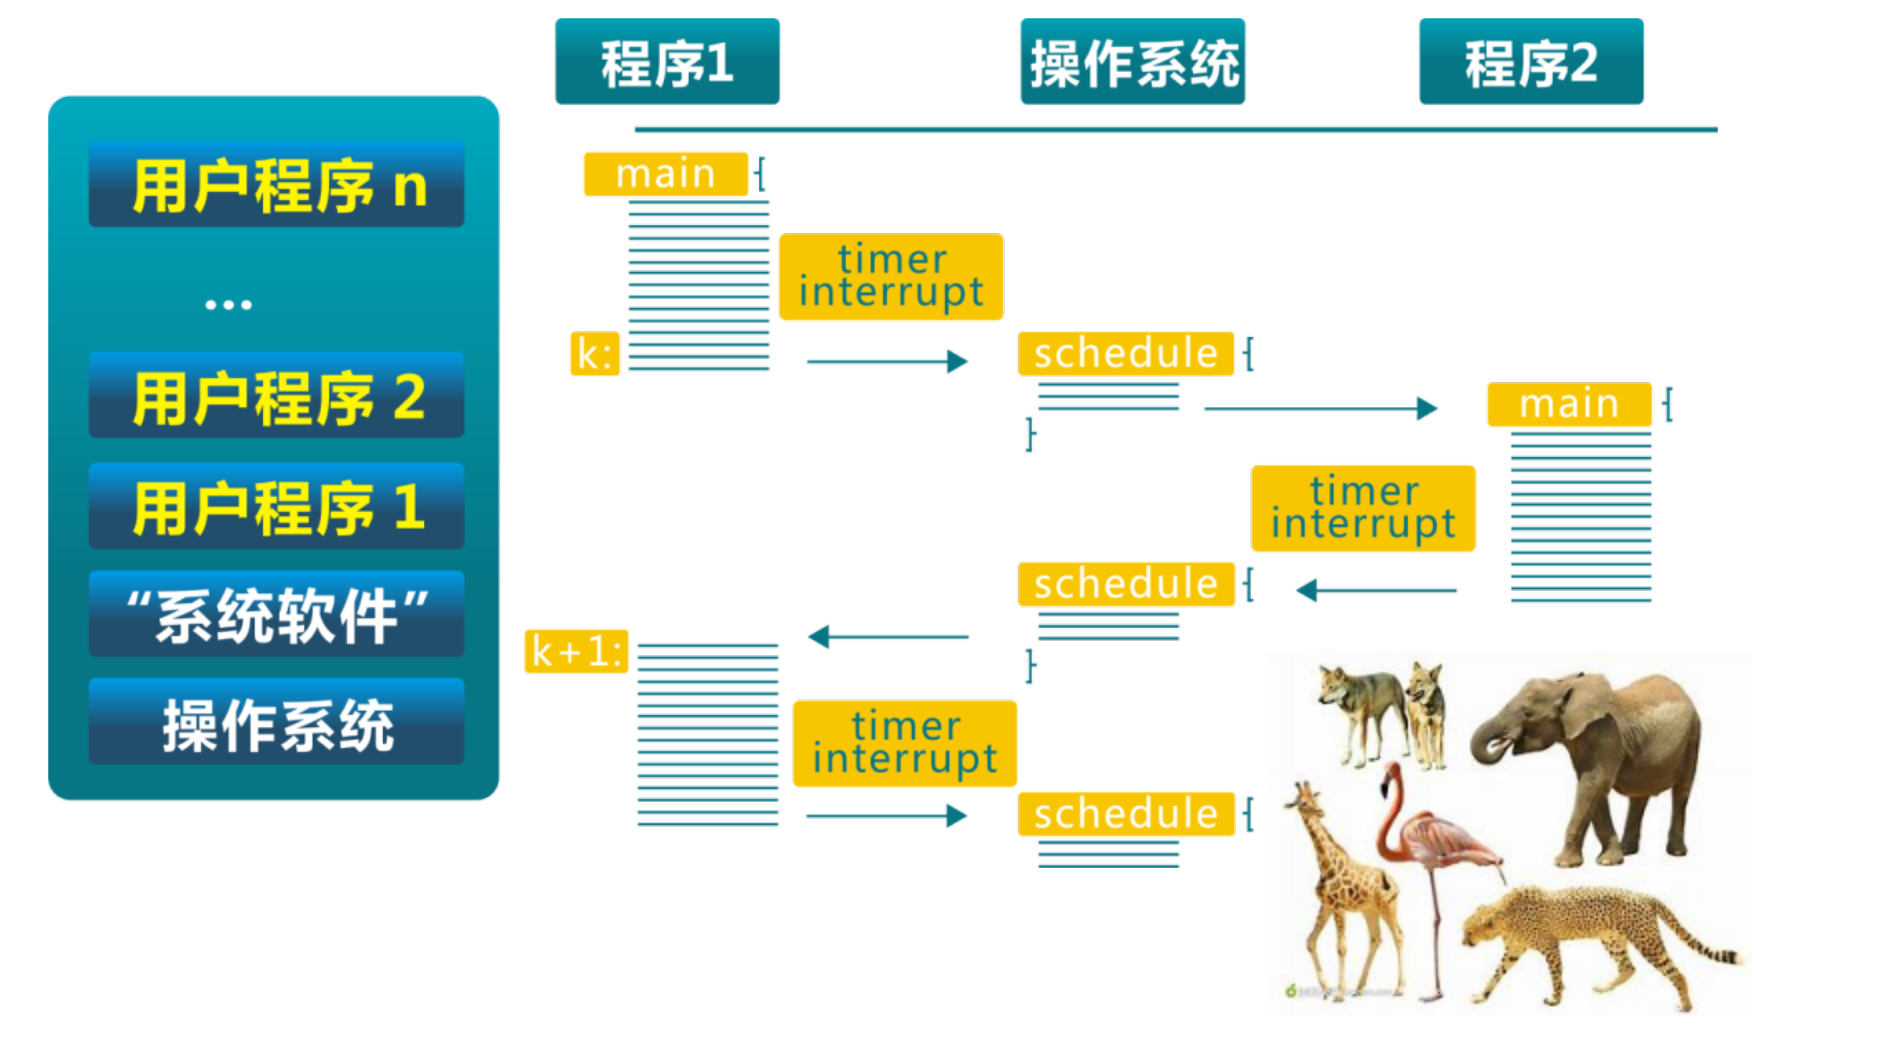
\includegraphics[width=0.6\linewidth]{history-timesharing}
		\caption{分时处理流程}
	\end{figure}
	
\end{frame}


\begin{frame}
	
	\frametitle{个人电脑}
	
	个人电脑(1981- )
	% 1981-8-12 · IBM型号IBM 5150电脑,售价1565美元 1981年08月12日国际商用机器公司(IBM)推出
	% 了型号为IBM5150的新款电脑,个人电脑这个新生市场从此诞生。
	\begin{itemize}
		\item 单用户
		\item CPU利用率已不再是最重要的关注点	
		\item 重点是用户界面和多媒体功能
		\item 操作系统=装载器+程序调度+内存管理+中断处理+...
		\item 演变:走向大众,老的服务和功能不存在,越来越多的安全问题
	\end{itemize}
	
	\begin{figure}
		\centering
		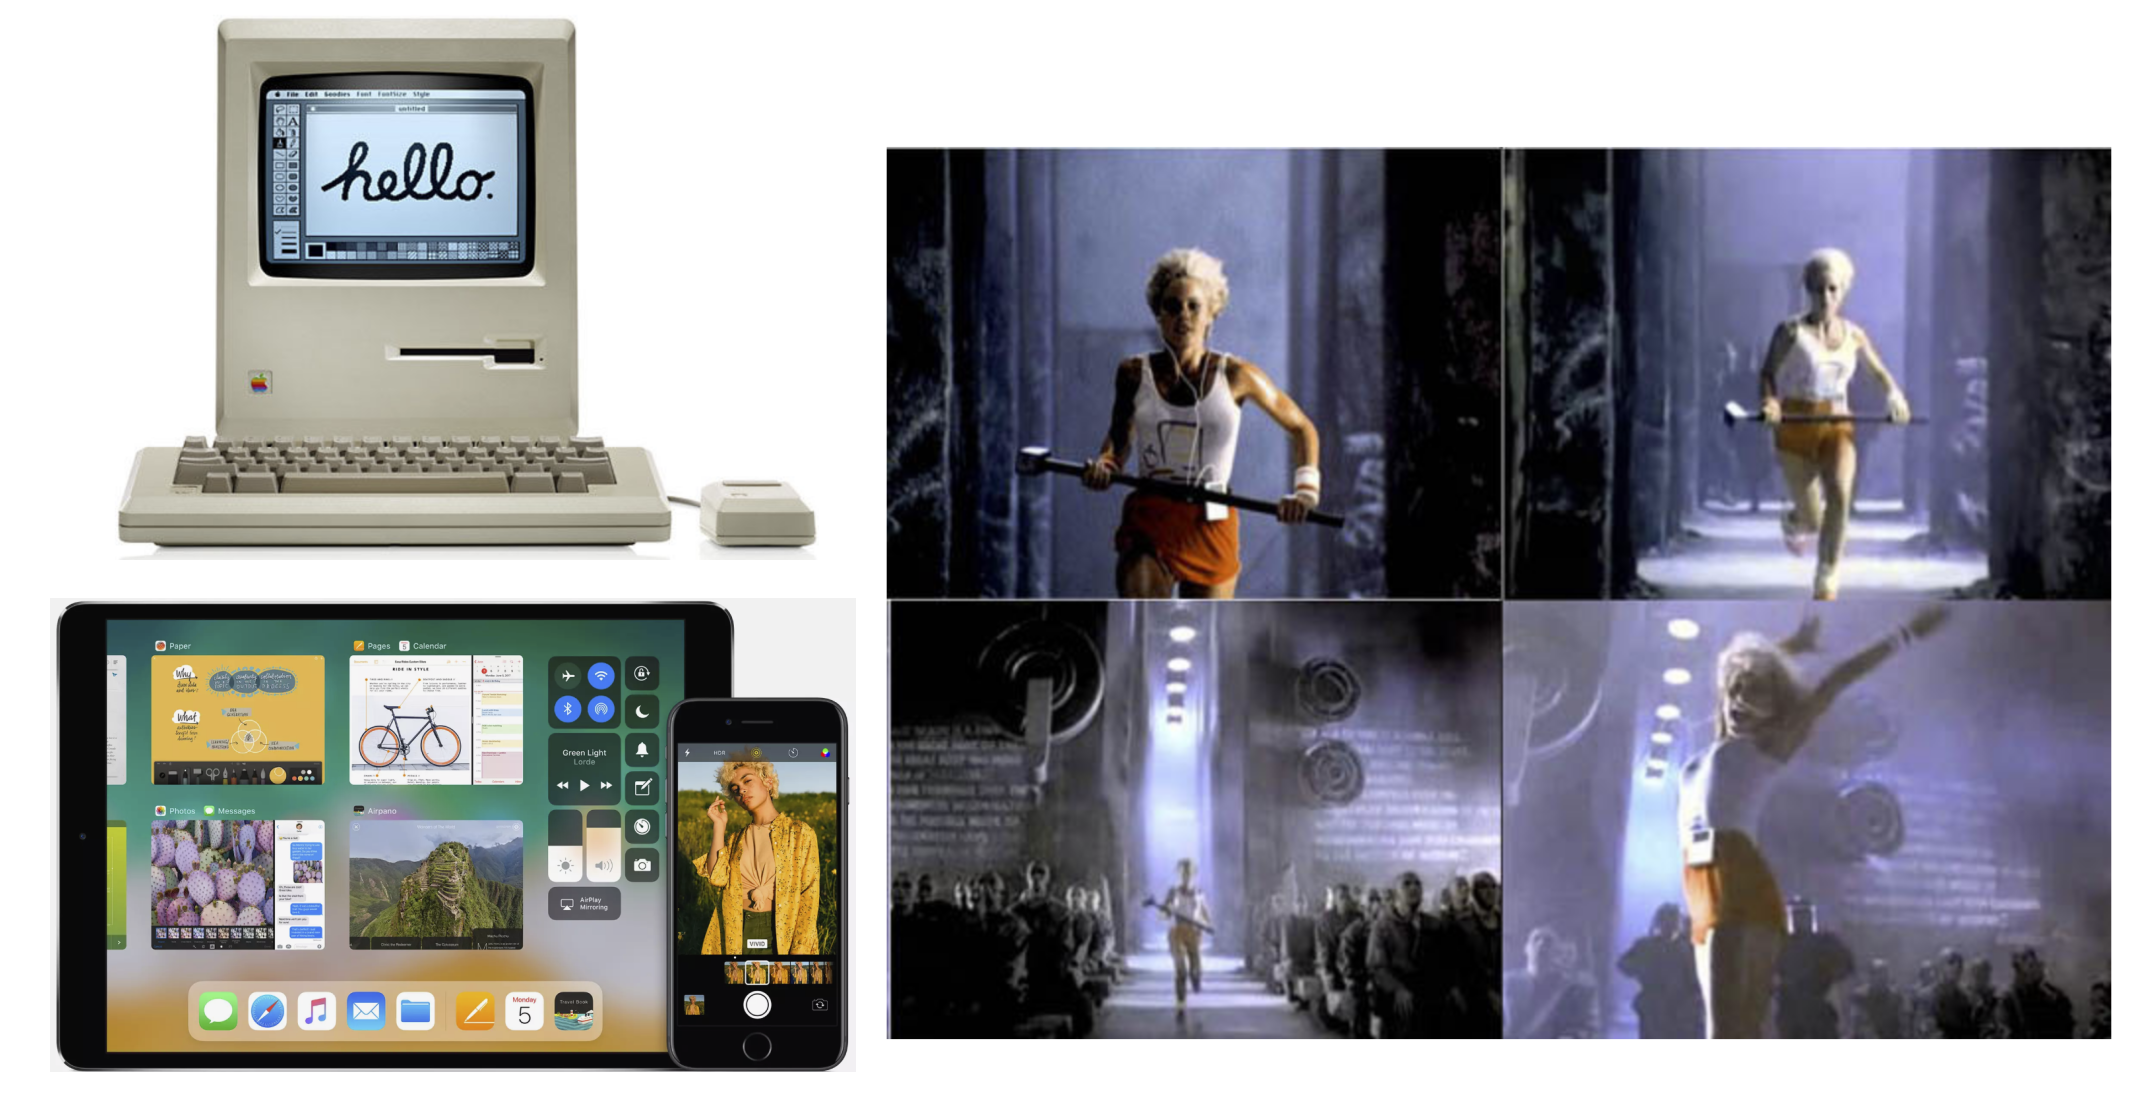
\includegraphics[width=0.6\linewidth]{history-pc}
		\caption{个人电脑}
	\end{figure}
	
\end{frame}



\begin{frame}
	
	\frametitle{分布式系统}
	
	分布式系统(1990- )

	\begin{itemize}
		\item 分布式多用户
		\item 分布式系统利用率是关注点	
		\item 重点是网络/存储/计算的效率
		\item 操作系统=分布式(装载器+程序/OS调度+内存管理)
		\item 演变:走向大众,走向网络,新的挑战(不可靠/不确定)
	\end{itemize}
	
	\begin{figure}
		\centering
		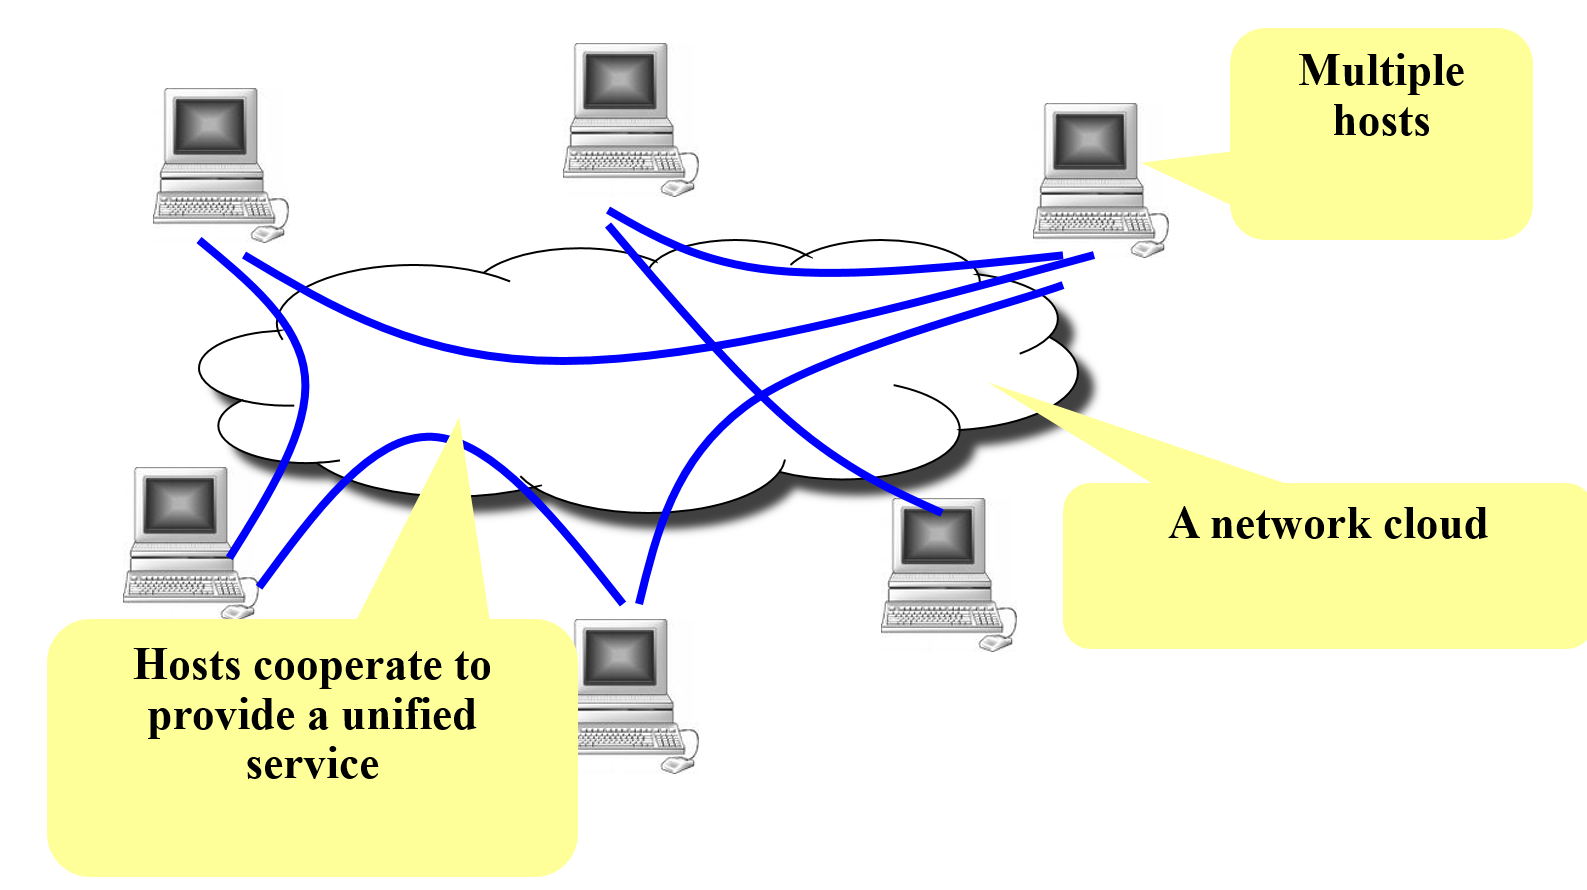
\includegraphics[width=0.6\linewidth]{history-ds}
		\caption{分布式系统}
	\end{figure}
	
\end{frame}

\begin{frame}
	
	\frametitle{AIoT系统}
	
	AIoT系统(2000- )

	\begin{itemize}
		\item 分布式多设备
		\item 分布式系统利用率/可用性是关注点	
		\item 重点是网络/存储/计算的效率
		\item 操作系统=分布式(程序/OS调度+内存管理+安全/更新)
		\item 演变:走向设备,走向网络,新的挑战(不可靠/大数据)
	\end{itemize}
	
	\begin{figure}
		\centering
		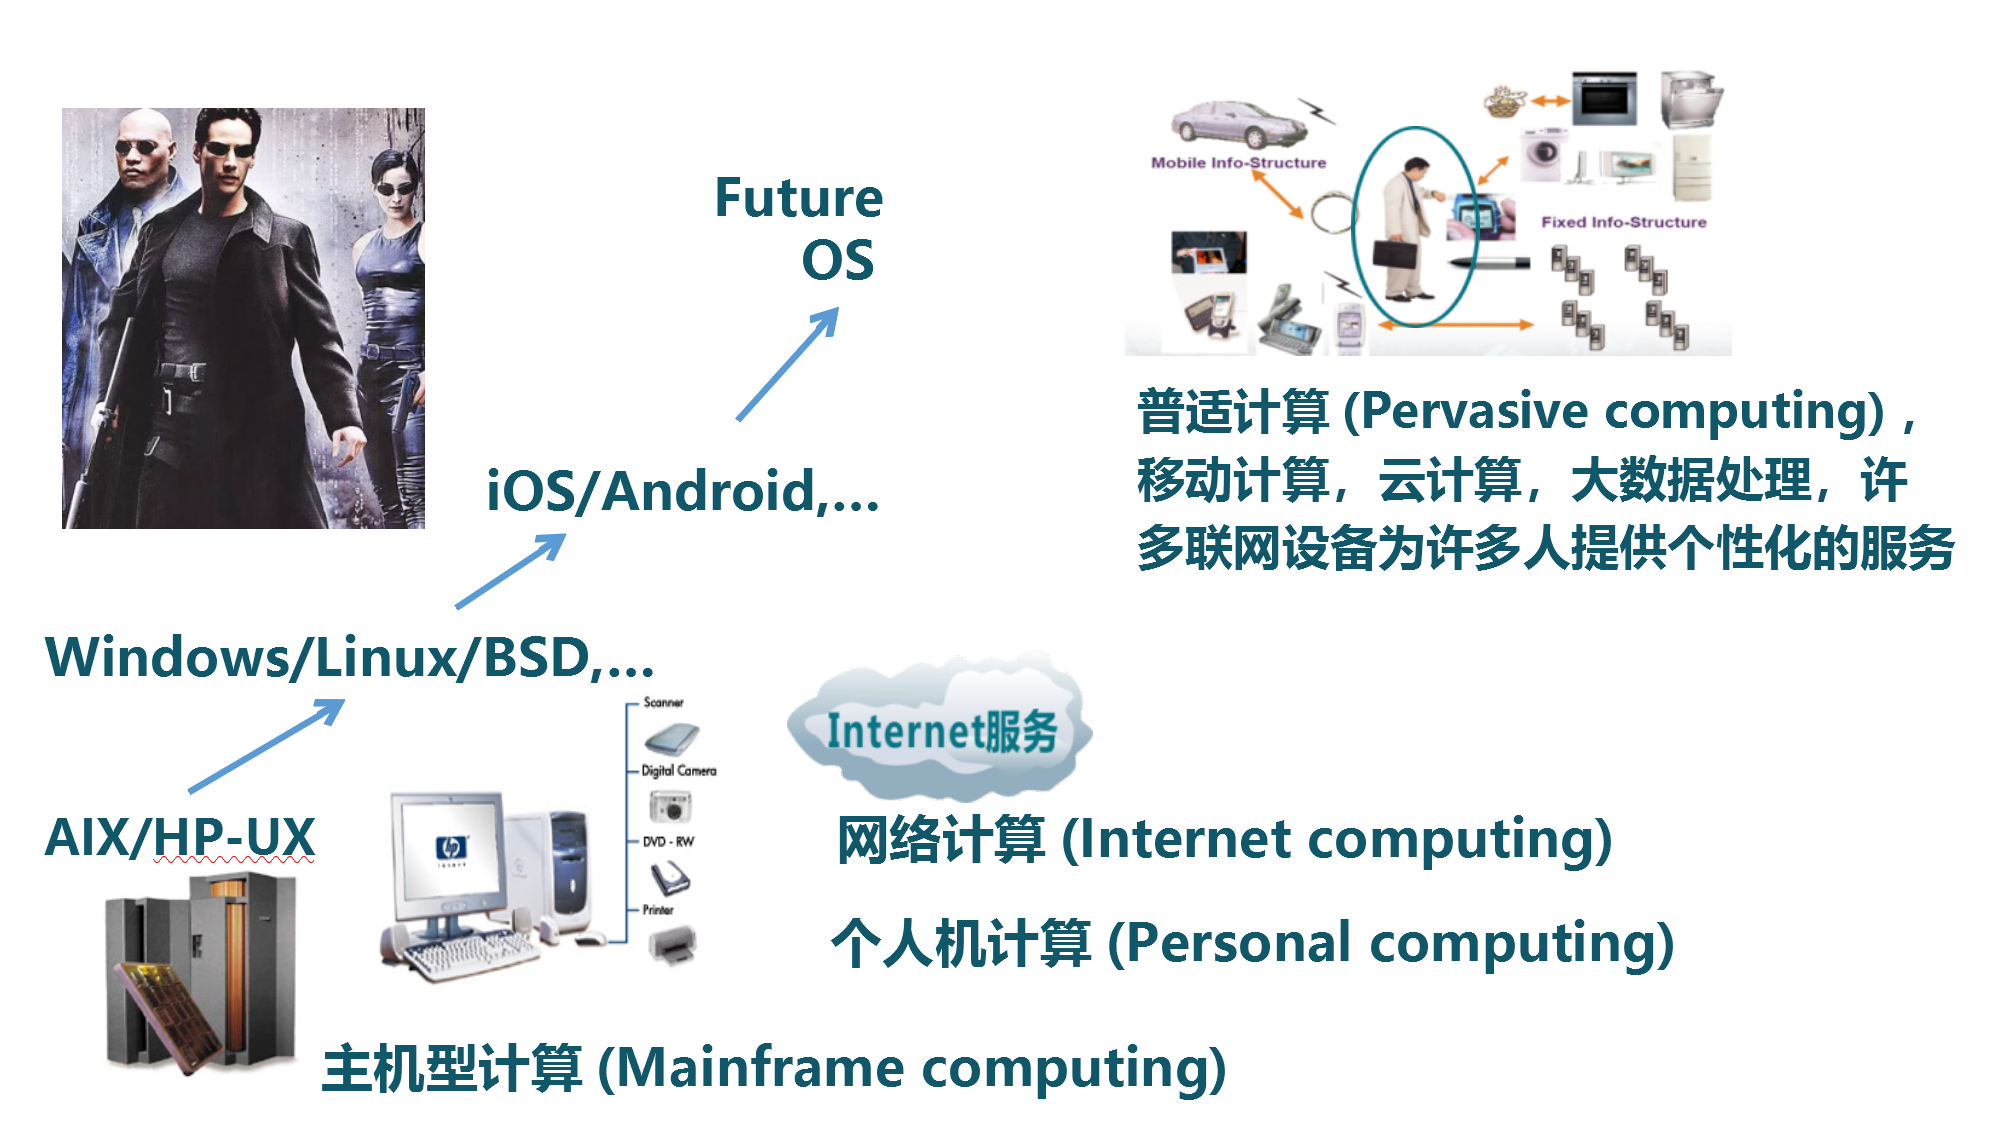
\includegraphics[width=0.6\linewidth]{history-aiot}
		\caption{AIoT系统}
	\end{figure}
	
\end{frame}

%----------------------------------------------------------------------------------------

\end{document}
